\documentclass[../../../../main.tex]{subfiles}
\usepackage{amsmath,amssymb,graphicx,tikz}
\usetikzlibrary{calc,patterns}

\begin{document}

\section*{東大理科数学 2007年}

\begin{center}
\begin{tabular}{|c|c|c|c|c|}
\hline
問 & 分野 & 計 & 思 & 総 \\ \hline
1 & & A & C & B \\ \hline
2 & & B & A & B \\ \hline
3 & & B & B & B \\ \hline
4 & 行列 & & & \\ \hline
5 & & B & A & A \\ \hline
6 & & B & B & B \\ \hline
\end{tabular}
\end{center}

\bigskip

\subsection*{第1問}

\begin{proof}[解]
$P(x)$ の $n$ 次以下の部分を $R_n(x)$, $Q_n(x) = (1+x)^k R_n(x)$ とおくと
「$Q_n(x)$ の $n$ 次以下の項の係数が $\mathbb{Z}$ に属する時, $R_n(x)$ の全ての項の係数も $\mathbb{Z}$ に属する」ことを示せば良い.
\[
R_n(x) = \sum_{i=0}^n a_i x^i
\]
\[
Q_n(x) = \sum_{i=0}^{n+k} b_i x^i \quad (b_i \text{ は } i=0,1,\dots,n+k \text{ の時整数}) \quad \cdots \star
\]
以下, $\star$ を $l$ についての帰納法で示す. $l=0$ の時,
$b_0 = a_0$ となり, $a_0 \in \mathbb{Z}$ だから成立する. 以下 $i \le l$ ($l=1,2,\dots,n-1$) での成立を仮定する.
\[
Q_n(x) = \left( x^k + k x^{k-1} + {}_k\mathrm{C}_2 x^{k-2} + \dots + kx + 1 \right) (a_n x^n + \dots + a_0)
\]
だから, $Q_n(x)$ の $l+1$ 次項は, $a_{l+1} + (\text{整数}) \quad (\because \text{仮定})$ の形で表せるから
\[
a_{l+1} = b_{l+1} - (\text{整数}) \in \mathbb{Z}
\]
となり, $i=l+1$ でも仮定は成立. 以上から示された. \quad \text{//}
\end{proof}

\subsection*{第2問}

\begin{proof}[解]
$n \in \mathbb{Z}_{\ge 2} \quad \cdots \text{\textcircled{ア}}$. $\angle OP_0 P_1 = \theta$, $OP_{k-1} = b_k$ とおく.

$\triangle O P_{k-1} P_k$ に正弦定理を用いる:

\begin{center}
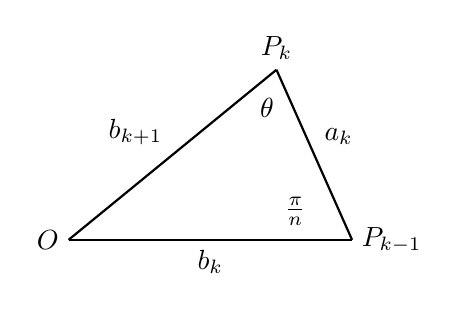
\begin{tikzpicture}[scale=1.2]
  \coordinate (O) at (0,0);
  \coordinate (Pk1) at (3,0);
  \coordinate (Pk) at (2.2, 1.8);
  \draw[thick] (O) -- (Pk1) node[midway, below] {$b_k$};
  \draw[thick] (O) -- (Pk) node[midway, above left] {$b_{k+1}$};
  \draw[thick] (Pk1) -- (Pk) node[midway, above right] {$a_k$};
  \node[left] at (O) {$O$};
  \node[right] at (Pk1) {$P_{k-1}$};
  \node[above] at (Pk) {$P_k$};
  \node at (2.4, 0.3) {$\frac{\pi}{n}$};
  \node at (2.1, 1.4) {$\theta$};
\end{tikzpicture}
\end{center}

\[
\frac{a_k}{\sin \frac{\pi}{n}} = \frac{b_{k+1}}{\sin \theta} = \frac{b_k}{\sin\left(\theta + \frac{\pi}{n}\right)} \quad \cdots ①
\]
①から
\[
b_{k+1} = \frac{\sin \theta}{\sin\left(\theta + \frac{\pi}{n}\right)} b_k \quad \cdots \text{\textcircled{イ}}
\]
又 ②から $b_1 = 1, b_2 = 1 + \frac{1}{n}$ だから, \textcircled{イ} で $k=1$ として

\begin{center}
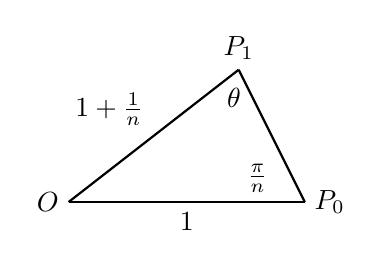
\begin{tikzpicture}[scale=1.2]
  \coordinate (O) at (0,0);
  \coordinate (P0) at (2.5,0);
  \coordinate (P1) at (1.8,1.4);
  \draw[thick] (O) -- (P0) node[midway, below] {$1$};
  \draw[thick] (O) -- (P1) node[midway, above left] {$1+\frac{1}{n}$};
  \draw[thick] (P0) -- (P1);
  \node[left] at (O) {$O$};
  \node[right] at (P0) {$P_0$};
  \node[above] at (P1) {$P_1$};
  \node at (2.0, 0.25) {$\frac{\pi}{n}$};
  \node at (1.75, 1.1) {$\theta$};
\end{tikzpicture}
\end{center}

\[
1 + \frac{1}{n} = \frac{\sin \theta}{\sin\left(\theta + \frac{\pi}{n}\right)} \quad \cdots \text{\textcircled{ウ}}
\]
\textcircled{イ}, \textcircled{ウ} と上記の初期条件から
\[
b_k = \left(1 + \frac{1}{n}\right)^{k-1} \quad \cdots \text{\textcircled{エ}}
\]
$\alpha = 1 + \frac{1}{n}$ として $\triangle O P_k P_{k-1}$ に余弦定理を用いて
\[
a_k = \alpha^{k-1} \sqrt{1 + \alpha^2 - 2\alpha \cos \frac{\pi}{n}}
\]
だから
\[
S_n = \frac{1 - \alpha^n}{1 - \alpha} \sqrt{1 + \alpha^2 - 2\alpha \cos \frac{\pi}{n}}
\]
$t = \frac{1}{n}$ とおいて整理する
\[
S_n = (\alpha^n - 1) \sqrt{ 2 \frac{1 - \cos t\pi}{t^2} + 1 + \frac{2(1 - \cos t\pi)}{t} }
\]
\[
\longrightarrow (e - 1) \sqrt{\pi^2 + 1} \quad (n \to \infty) \quad \text{//}
\]
\end{proof}

\subsection*{第3問}

\begin{proof}[解]
(1) $P(\alpha, \alpha^2), Q(\beta, \beta^2) \quad (-1 \le \alpha \le \beta \le 1)$ とおいて良い. $R(a, b)$ とすると
\[
a = \frac{1}{3}(2\alpha + \beta), \quad b = \frac{1}{3}(2\alpha^2 + \beta^2)
\]
前者から $\beta$ を消去して $\beta = 3a - 2\alpha$ だから, 後者, 定義域に代入
\[
-1 \le 3a - 2\alpha \le 1 \quad \cdots ①
\]
\[
b = \frac{1}{3} \left[ 2\alpha^2 + (3a - 2\alpha)^2 \right] = 2\alpha^2 - 4a\alpha + 3a^2 \equiv f(\alpha) \quad \cdots ②
\]
以下, ① の $-1 \le \alpha \le 1$ のもとで $b$ のとりうる値を調べる.

\begin{center}
\begin{tikzpicture}[scale=2]
  \draw[->] (-1.3,0) -- (1.3,0) node[right] {$a$};
  \draw[->] (0,-1.3) -- (0,1.3) node[above] {$\alpha$};
  
  \fill[gray!20] (-1,-1) -- (-1/3,-1) -- (1,1) -- (1/3,1) -- cycle;
  \draw[thick] (-1,-1) -- (-1/3,-1) -- (1,1) -- (1/3,1) -- cycle;
  
  \draw[dashed] (-1.2,-1.2) -- (1.2,1.2) node[above right] {軸: $\alpha = a$};
  \draw[dashed] (-1, -1) -- (1/3, 1) node[above] {$\alpha = \frac{1}{2}(3a+1)$};
  \draw[dashed] (-1/3, -1) -- (1, 1) node[right] {$\alpha = \frac{1}{2}(3a-1)$};
  
  \node[below] at (-1,0) {$-1$};
  \node[below] at (-1/3,0) {$-\frac{1}{3}$};
  \node[below] at (1/3,0) {$\frac{1}{3}$};
  \node[below] at (1,0) {$1$};
  
  \node[left] at (0,-1) {$-1$};
  \node[left] at (0,1) {$1$};
  \node[below left] at (0,0) {$O$};
\end{tikzpicture}
\end{center}

\[
\begin{cases}
-1 \le a \le -\frac{1}{3} \text{ の時 } f(a) \le b \le f(-1) \\
-\frac{1}{3} \le a \le 0 \text{ の時 } f(a) \le b \le f\left(\frac{3a-1}{2}\right) \\
0 \le a \le \frac{1}{3} \text{ の時 } f(a) \le b \le f\left(\frac{3a+1}{2}\right) \\
\frac{1}{3} \le a \le 1 \text{ の時 } f(a) \le b \le f(1)
\end{cases}
\]
$\iff$
\[
\begin{cases}
-1 \le a \le -\frac{1}{3} \text{ の時 } a^2 \le b \le 3a^2 + 4a + 2 \\
-\frac{1}{3} \le a \le 0 \text{ の時 } a^2 \le b \le \frac{3}{2}a^2 - a + \frac{1}{2} \\
0 \le a \le \frac{1}{3} \text{ の時 } a^2 \le b \le \frac{3}{2}a^2 + a + \frac{1}{2} \\
\frac{1}{3} \le a \le 1 \text{ の時 } a^2 \le b \le 3a^2 - 4a + 2
\end{cases}
\quad \cdots \text{\textcircled{井}}
\]

\begin{center}
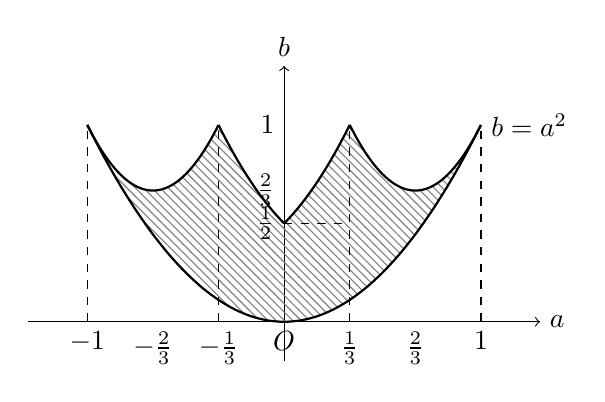
\begin{tikzpicture}[scale=2.5]
  \draw[->] (-1.3,0) -- (1.3,0) node[right] {$a$};
  \draw[->] (0,-0.2) -- (0,1.3) node[above] {$b$};
  
  \fill[pattern=north west lines, pattern color=gray] 
    plot[domain=-1:-1/3, smooth] (\x, {3*\x*\x + 4*\x + 2}) --
    plot[domain=-1/3:0, smooth] (\x, {1.5*\x*\x - \x + 0.5}) --
    plot[domain=0:1/3, smooth] (\x, {1.5*\x*\x + \x + 0.5}) --
    plot[domain=1/3:1, smooth] (\x, {3*\x*\x - 4*\x + 2}) --
    plot[domain=1:-1, smooth] (\x, {\x*\x}) -- cycle;

  \draw[thick, domain=-1:1, smooth] plot (\x, {\x*\x}) node[right] {$b = a^2$};
  \draw[thick, domain=-1:-1/3, smooth] plot (\x, {3*\x*\x + 4*\x + 2});
  \draw[thick, domain=-1/3:0, smooth] plot (\x, {1.5*\x*\x - \x + 0.5});
  \draw[thick, domain=0:1/3, smooth] plot (\x, {1.5*\x*\x + \x + 0.5});
  \draw[thick, domain=1/3:1, smooth] plot (\x, {3*\x*\x - 4*\x + 2});
  
  \draw[dashed] (-1,0) -- (-1,1);
  \draw[dashed] (-1/3,0) -- (-1/3,1);
  \draw[dashed] (1/3,0) -- (1/3,1);
  \draw[dashed] (1,0) -- (1,1);
  \draw[dashed] (0,0.5) -- (0.33,0.5);
  
  \node[below] at (-1,0) {$-1$};
  \node[below] at (-2/3,0) {$-\frac{2}{3}$};
  \node[below] at (-1/3,0) {$-\frac{1}{3}$};
  \node[below] at (0,0) {$O$};
  \node[below] at (1/3,0) {$\frac{1}{3}$};
  \node[below] at (2/3,0) {$\frac{2}{3}$};
  \node[below] at (1,0) {$1$};
  
  \node[left] at (0,1) {$1$};
  \node[left] at (0,2/3) {$\frac{2}{3}$};
  \node[left] at (0,1/2) {$\frac{1}{2}$};
\end{tikzpicture}
\end{center}
\end{proof}

\subsection*{第4問}

（解答なし）

\subsection*{第5問}

\begin{proof}[解]
$n \in \mathbb{N}, 0 \le m \le n, m \in \mathbb{Z} \quad \cdots ①$

(1) $n$ 回投げて $m$ となるのは以下の時. ($1 \le m \le n-1$)
\[
\circ \quad \dots \quad \underbrace{\circ}_{\text{↑ } n-m-1 \text{ 回目ウラ}} \quad \underbrace{\circ}_{\text{↑ } n-m \text{ 回目表}} \quad \dots \quad \circ
\]
$m=n$ の時, $n$ 回とも表で, $P_n = p^n$. $m=0$ の時, $n$ 回目がウラで, $P_0 = 1-p$.
$1 \le m \le n-1$ の時, 上図から $P_m = (1-p) p^m$ で, $m=0$ の時もこれで良い.
\[
P_m = \begin{cases} p^n & (m = n) \\ (1-p) p^m & (m \neq n) \end{cases}
\quad \text{\#}
\]

(2) $q_m = \sum_{k=0}^m P_k$ である. $m=0$ の時, $q_0 = 1-p$. $m \ge 1$ の時,
\[
q_m = \sum_{k=0}^{m-1} P_k + P_m = (1-p) \frac{1-p^m}{1-p} + P_m
\]
だから, $m=n$ か否かで場合分けし, $m=0$ の時もこれで良いから
\[
q_m = \begin{cases} 1 - p^{m+1} & (m \neq n) \\ 1 & (m = n) \end{cases}
\quad \text{\#}
\]

(3) 2つのブロックを $A, B$ とおく. また, $A, B$ の高さを $a, b$ で表す. 包除原理から,
\[
r_m = P(a=m \cap b \le m) + P(b=m \cap a \le m) - P(a=b=m)
\]
\[
= 2 P_m q_m - P_m P_m \quad \cdots ②
\]
である.

$\cdot$ $m=n$ の時
②及び(1),(2)から
\[
r_n = p^n (2 - p^n)
\]

$\cdot$ $m \neq n$ の時
$1^\circ$ と同様にして
\[
r_m = (1-p)p^m \{ 2(1 - p^{m+1}) - (1-p)p^m \} = (1-p)p^m (2 - p^m - p^{m+1})
\]

以上から,
\[
r_m = \begin{cases} p^n (2 - p^n) & (m = n) \\ (1-p)p^m (2 - p^m - p^{m+1}) & (m \neq n) \end{cases}
\quad \text{\#}
\]
\end{proof}

\paragraph{[(3) 別解]}
\[
r_m = \begin{cases} q_m^2 - q_{m-1}^2 & (m \ge 1) \\ q_0^2 & (m = 0) \end{cases}
\]
だから, (2) から計算できる (以下略).

\subsection*{第6問}

\begin{proof}[解]
(1) $y = \frac{1}{t}$ のグラフは $t > 0$ の時, 下に凸だから, 右図で面積を比較して ($\because a-x > 0$)

\begin{center}
\begin{tikzpicture}[scale=2]
  \draw[->] (-0.2,0) -- (3,0) node[right] {$t$};
  \draw[->] (0,-0.2) -- (0,2.5) node[above] {$y$};
  
  \draw[domain=0.5:2.5, smooth, variable=\t, blue, thick] plot ({\t}, {1.8/\t}) node[right] {$y = \frac{1}{t}$};
  
  \coordinate (P) at (0.8, {1.8/0.8});
  \coordinate (A) at (1.4, {1.8/1.4});
  \coordinate (B) at (2.0, {1.8/2.0});
  
  \draw[dashed] (0.8,0) node[below] {$a-x$} -- (P);
  \draw[dashed] (1.4,0) node[below] {$a$} -- (A);
  \draw[dashed] (2.0,0) node[below] {$a+x$} -- (B);
  
  \draw[red, thick] (0.6, {1.8/1.4 - (-0.918)*(0.6-1.4)}) -- (2.2, {1.8/1.4 - (-0.918)*(2.2-1.4)}) node[right] {点Aでの接線};
  
  \draw[green!60!black, thick] (P) -- (B);
  
  \fill (P) circle (1pt) node[above left] {$P$};
  \fill (A) circle (1pt) node[above right] {$A$};
  \fill (B) circle (1pt) node[right] {$B$};
  \node[left] at (0, {1.8/1.4}) {$\frac{1}{a}$};
\end{tikzpicture}
\end{center}

\[
\text{台形} ABCD < \int_{a-x}^{a+x} \frac{1}{t} dt < \text{台形} ABEF
\]
だから
\[
\frac{2x}{a} < \int_{a-x}^{a+x} \frac{1}{t} dt < x \left( \frac{1}{a-x} + \frac{1}{a+x} \right) \quad \text{\#}
\]

(2) (1) と同様の評価を $[a-x, a]$, $[a, a+x]$ で行うことで以下の不等式を得る.
\[
\frac{x}{a - \frac{x}{2}} < \int_{a-x}^a \frac{1}{t} dt < \frac{1}{2} x \left( \frac{1}{a} + \frac{1}{a-x} \right)
\]
\[
\frac{x}{a + \frac{x}{2}} < \int_a^{a+x} \frac{1}{t} dt < \frac{1}{2} x \left( \frac{1}{a} + \frac{1}{a+x} \right)
\]
辺々足して,
\[
2x \left( \frac{1}{2a-x} + \frac{1}{2a+x} \right) < \int_{a-x}^{a+x} \frac{1}{t} dt < \frac{1}{2} x \left( \frac{2}{a} + \frac{1}{a-x} + \frac{1}{a+x} \right) \quad \cdots ①
\]
この中辺は $\log \frac{a+x}{a-x}$ であることに注意し, $a=3x$ ($0 < x < a$) を ① に代入し,
\[
\frac{2}{5} + \frac{2}{7} < \log 2 < \frac{1}{2} \left( \frac{2}{3} + \frac{3}{4} \right)
\]
\[
\frac{24}{35} < \log 2 < \frac{17}{24} \quad \cdots ②
\]
ここで,
\[
\frac{24}{35} - \frac{68}{100} = \frac{1}{5} \left( \frac{24}{7} - \frac{17}{5} \right) = \frac{1}{5} \cdot \frac{1}{35} > 0 \quad \therefore 0.68 < \frac{24}{35}
\]
\[
\frac{71}{100} - \frac{17}{24} = \frac{1}{600} (426 - 425) = \frac{1}{600} > 0 \quad \therefore 0.71 > \frac{17}{24}
\]
だから, ① とあわせて
\[
0.68 < \log 2 < 0.71 \quad \text{\#}
\]
\end{proof}

\paragraph{[(2) 別解]}
（なぜか中点を $\log 2$ にすると解決する）
$x = (3 - 2\sqrt{2})a$ と推測（条件をみたす！）. (1) に代入して
\[
6 - 4\sqrt{2} < \frac{1}{2} \log 2 < \frac{15}{64}
\]
\[
4(3 - 2\sqrt{2}) < \log 2 < \frac{1}{2}
\]
$1.415 < \sqrt{2} < 1.42$ を示して用いることで, 所望の不等式を得る.

\begin{center}
\begin{tikzpicture}[scale=1.8]
  \draw[->] (-0.2,0) -- (2.5,0) node[right] {$t$};
  \draw[->] (0,-0.2) -- (0,2) node[above] {$y$};
  \draw[domain=0.5:2.2, smooth, variable=\t, blue, thick] plot ({\t}, {1.5/\t});
  \draw[dashed] (0.8,0) node[below] {$a-x_2$} -- (0.8, {1.5/0.8});
  \draw[dashed] (1.2,0) node[below] {$a-x_1$} -- (1.2, {1.5/1.2});
  \draw[dashed] (1.6,0) node[below] {$a$} -- (1.6, {1.5/1.6});
  \node at (1.0, 1.2) {誤差};
\end{tikzpicture}
\end{center}
$x_1 = (3-2\sqrt{2})a$, $x_2 = \frac{1}{3}a$ において,
$x_1 < x_2$ となっているので, グラフを考えると, 明らかに $x_1$ の方が正確な評価（近似）になっている, という仕掛けかな.

\end{document}
